\chapter{Models}
	This chapter presents an assortment of approaches that have been used to attempt to model combat. Ultimately, these are all approximations. Thankfully, an exact solution can be found through a Markov Chain analysis, which will be presented in the next chapter. The models here vary in how they handle overkill and they will be presented roughly in order of increasing complexity. They operate under the following assumptions:
	\begin{enumerate}
		\item A successful attack is uniformly distributed between $[0, M]$ (noting there are $M+1$ integers in this range).
		\item An attack is successful with the probability $a\in[0, 1]$, which is the attacker's accuracy.
		\item The defender starts at a health $h_0$.
		\item Attacks occur every $T_A$ seconds.
		\item No special attacks, or weapon switches are considered.
		\item The first attack occurs at time, $t=0$ or attack number $n=0$ depending on context.
		\item If health regeneration is considered, it occurs every $T_r$, and heals one health.
				The first regeneration will occur as a uniform random variable at $t\sim U[0, T_r]$.
	\end{enumerate}
	There are two relevant quantities that will be calculated for each model: time to health, and health after time.

	There are some basic results we can already state:
	\begin{enumerate}
		\item The number of attack attempts is simply $a$ times the number of successful attacks.
		\item The time taken for $n$ attacks is simply $nT_A$.
	\end{enumerate}



	Only the last model will discuss health regeneration, and it will take a non-regeneration model as input so it applies generally.
	Finally, a comparison between the different models will be performed.


	\section{Crude Model}
		\subsection{Health after \texorpdfstring{$n$}{} attacks}
			This model does not consider overkill and as a result is very straight forward. The average damage per successful attack is,
			\begin{align}
				\langle D \rangle &= \frac{1}{M+1}\sum_{i=0}^M i\\
					&= \frac{1}{\cancel{M+1}} \frac{M\cancel{(M+1)}}{2}\\
					&= \frac{M}{2}.
			\end{align}
			After each attack, the health will lower by this amount, recursively this allows us to state:
			\begin{equation}
				h_{n+1} = h_{n} - \langle D \rangle,\,\,\,h_0\equiv\text{Initial Health}.
			\end{equation}
			In this case the health after $n$ successful attacks is:
			\begin{align}
				h_{n+1} &= h_{n} - \frac{M}{2}\\
				\Aboxed{h_{n} &= h_0 - n\frac{M}{2}}.
			\end{align}
		\subsection{Attacks until \texorpdfstring{$h$}{} health}
			This equation can be inverted to give the number of turns to a given health,
			\begin{align}
				\Aboxed{n &= (h_0 - h_{n}) \frac{2}{M}}.
			\end{align}
			Both of these can be calculated in $\mathcal{O}(1)$ time.
	
	\section{Average}
		\subsection{Average Damage}
			\href{https://imgur.com/aykEahg}{Nukelawe} presents a derivation that gives the average damage per hit over the opponent's life to be. This means a contribution from the overkill region and a contribution from the normal region. This averaging acts as an approximation since adds each hit in the overkill region, however in reality only a couple hits during a fight would occur here. With this, the average damage on a hit is given by:
			\begin{align}
				\langle D \rangle_{h_0}^M = \frac{y(y+1)}{h_0(M+1)}\left(\frac{1}{2}{(M+h_0+1)}-\frac{1}{3}(2y+1) \right),
			\end{align}
			where $y=\min(h_0, M)$. Since this is an average over the length of a fight, it means that we cannot determine the health after a given number of terms for this model.


			% \begin{align}
			% 	\Aboxed{h_{n} &= h_0 - n\frac{y(y+1)}{h_0(M+1)}\left(\frac{1}{2}{(M+h_0+1)}-\frac{1}{3}(2y+1) \right)}.
			% \end{align}

		\subsection{Attacks to kill}
			Since we know the average damage over the whole fight, we can calculate the number of attacks to kill simply by,
			\begin{align}
				n &= \frac{h_0}{\langle D \rangle} \\
				&= \frac{h^2_0(M+1)}{y(y+1)}\frac{6}{\left(3M+3h_0+3-4y-2) \right)} \\
				\Aboxed{n &= \frac{6h^2_0(M+1)}{y(y+1)\left(3M+3h_0-4y+1) \right)}}
			\end{align}
			This can be calculated in $\mathcal{O}(1)$ time.

	\section{Recursive Model}\label{sec:average_damage}
		\subsection{Expected Damage per Hit}
			The Crude model made the assumption that the player can always hit up to their max hit. This is not the case if the opponent has less health, $h$ than the maximum hit.
			\begin{center}
			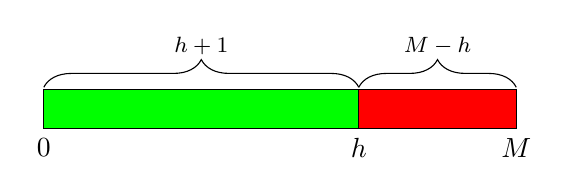
\begin{tikzpicture}
				\filldraw[fill=green, draw=black] (0,0) node[anchor=north] {$0$} -- (4,0) node[anchor=north] {$h$} -- (4,0.5) -- (0,0.5) -- (0,0);
				\filldraw[fill=red, draw=black] (4,0) -- (6,0) node[anchor=north] {$M$} -- (6,0.5) -- (4,0.5) -- (4,0);
				\draw [decorate,decoration={brace,amplitude=10pt},xshift=0pt,yshift=15pt]
				(0,0) -- (4,0) node [black,midway,yshift=15pt]{
					\footnotesize $h+1$
				};
				\draw [decorate,decoration={brace,amplitude=10pt},xshift=0pt,yshift=15pt]
				(4,0) -- (6,0) node [black,midway,yshift=15pt]{
					\footnotesize $M-h$
				};
			\end{tikzpicture}
			\end{center}
			Considering this, we could hit every integer below $h$ each with a probability of $1/(M+1)$, and we could hit exactly $h$ (since we're considering hits capped by $h$) with a probability of $(M-h)/(M+1)$. Averaging the expectations gives,
			\begin{align}
				\langle D \rangle_{h < M} &= \frac{1}{M+1}\sum_{i=0}^{h} i + \frac{M-h}{M+1}h \\
				&= \frac{1}{M+1}\frac{h(h+1)}{2} + \frac{M-h}{M+1}h \\
				&= \frac{h}{2}\frac{2M-h+1}{M+1}\\
				&= \frac{h}{2}\left(1 + \frac{M - h}{M+1}\right)\\
				&= \frac{h}{2}\left(2 - \frac{h + 1}{M+1}\right)
				% &= \frac{h^2}{2m} + \frac{h}{2m} + h - \frac{h^2}{m} \\
				% &= -\frac{h^2}{2m} + \left(\frac{1}{2m} + 1\right)h \\
			\end{align}

			Overall then, our expected damage on a successful hit is:
			\begin{align}
				\boxed{
					\langle D \rangle = \frac{1}{2}\begin{cases}
						M &\text{if $h \ge M$} \\
						h\left(2 - \frac{h + 1}{M+1}\right) &\text{if $h < M$} \\
					\end{cases}
				}
			\end{align}

			\begin{figure}
				\centering
				\includegraphics[width=\linewidth]{results/part_II/average_damage.pdf}
				\caption{The average damage of an attack with a maximum hit of $M$ on an opponent with $h$ health. The black line is the piecewise boundary.}
				\label{fig:average_d}
			\end{figure}


			This is plotted in Fig.~\ref{fig:average_d}. The Nukelawe model averages over these contributions for the \emph{overall} (i.e. not piecewise) expected hit, assuming each starting health is equally likely. This isn't totally accurate, regardless, it is good to check that our equations agree under this assumption:
			\begin{align}
				\langle D \rangle_\text{overall} &= \left \langle \langle D \rangle_{h < M} + \langle D\rangle_{h\ge M} \right \rangle\\
				&= \frac{1}{h_0}\left(\sum_{h<M} \langle D \rangle_{h < M} + \sum_{h\ge M}\langle D\rangle_{h\ge M} \rangle \right)\\
				&= \frac{1}{h_0}\left(
					\sum_{n=M+1}^{h_{0}}\frac{M}{2} +
					\sum_{n=1}^{y} \frac{n}{2}\left(2 - \frac{n + 1}{M+1}\right)
				\right) \\
				&= \frac{y(y+1)}{h_0(M+1)}\left(\frac{1}{2}{(M+h_0+1)}-\frac{1}{3}(2y+1) \right),
			\end{align}
			where $y=\min(M, h_0)$. The last step is actually quite tricky and involved to show. For that reason it can be found in Appendix~\ref{combat-app:power_reduction}. This agrees with Nukelawe's findings.

		\subsection{Health after \texorpdfstring{$n$}{} attacks}
			Despite the above being an ``average'', it is not the average damage expected per hit over the life time of an opponent since certain healths are much more likely to appear than others. As an example, suppose there is an opponent with 100 health fighting an attacker with a max hit of 30. On the first hit, the most likely health is 85. This means that unlike the above calculation, each hit is \emph{not} equally likely. Particularly, this over estimates the contribution in the overkill region, since (depending on the circumstances) let's say 1 or 2 hits is expected per kill. Those 1 or 2 hits are more likely to occur at specific $h$ values, but the average sums across all $h$ equally. In the non-overkill region, this has no impact due to it being constant. The proper treatment is to use the piecewise damage expectation in the recursive definition:
			\begin{align}
				h_{n+1} = h_{n} - \frac{1}{2}\begin{cases}
					M &\text{if $h_n \ge M$} \\
					h_n\left(2 - \frac{h_n + 1}{M+1}\right) &\text{if $h_n < M$}.
				\end{cases}
			\end{align}
			This however is too cumbersome to handle at once. Since the health is a decreasing monotonic function, we can consider it in two parts. While $h$ is above or equal to $M$ the solution to the above is the same as the Crude model's,
			\begin{align}
				h_n = h_0 - n\frac{M}{2}.\label{eq:h_crude}
			\end{align}
			The solution to the other is a bit more complex. After a certain number of iterations the health will drop below $M$ and the second case above will kick in. We'll say this occurs after $L$ iterations (noting that this \emph{average} quantity can be a non-integer),
			\begin{align}
				M &> h_0 - L\frac{M}{2} \\
				\frac{2}{M}(h_0 - M) &< L \\
				\implies L &= 2\left(\frac{h_0}{M} - 1\right).
			\end{align}
			Now the expected health that the second condition starts at is given by,
			\begin{align}
				\langle h_L \rangle &= h_0 - 2\left(\frac{h_0}{M} - 1\right) \frac{M}{2}\\
				&= M.
			\end{align}
			Thus the second case is expected to starts on iteration $L$ with an initial health of $M$. For simplicity, we will define $m\equiv n-L$. Returning to our recursive function,
			\begin{align}
				h_{m+1} &= h_{m} - \frac{h_m}{2}\left(2 - \frac{h_m + 1}{M+1}\right) \\
				&= h_{m} - h_m + \frac{h_m}{2}\frac{h_m + 1}{M+1} \\
				&= \frac{h_m^2 + h_m}{2(M+1)} \\
				h_{m+1} &= \gamma (h_m^2 + h_m), \label{eq:recur}
			\end{align}
			where $\gamma\equiv1 / 2(M+1)$. This type of recurrence relation is called a \href{http://mathworld.wolfram.com/QuadraticMap.html}{Quadratic Map}, and unfortunately it has no closed form solution in general. For the sake of completeness, we will call the solution to Eq.~\ref{eq:recur} $f(m; M, f_0)$. At this point we're left with,
			\begin{align}
					h(n; h_0, M) &=  \begin{cases}
					h_0 - \frac{1}{2}nM &\text{else if $n \le L$} \\
					f(n - L; M, M) &\text{otherwise}.
				\end{cases}
			\end{align}

			In general, we are more interested in the number of iterations that is required to kill an opponent which is the inverse of this function, $n=h^{-1}(h; h_0, M)$. However, since the recurrence relation cannot be solved analytically, we cannot obtain a general expression for this. We could numerically compute this result. However remember that we are dealing with \emph{expectation values} or averages. This means it is totally possible for the inverted function to say ``The opponents health will be 18 in 4.5 iterations, on average''. This is a problem because our recursive equation can only increment the iteration by one (and we can only start at $f_0$)! In the next section, we will look at an approximation that will allow us to handle non-integer expectations.

	\subsubsection{Approximate Solution}
			Despite not being able to find a closed-form solution for Eq.~\ref{eq:recur}, we can look for approximate solutions. Although it's rare, there are a few quadratic recurrence relations that \textbf{do} have solutions. There are two relevant cases, ones where a constant term is introduced, or ones where the linear term is removed. Since increasing $n$ (and therefore iterations) results in smaller and smaller $h_n$, it suggests that adding constant terms will heavily skew the results in this region. Removing the linear term is still not ideal since its contribution increases relative to the quadratic term, in the low $h_n$ limit (when this recursive case is required). However this should be less significant and we'll find that it does pretty well! If this justification does not satisfy you, please check out Appendix~\ref{combat-app:recursive_justification}. With this approximation, our recursive relation becomes,
			\begin{align}\label{eq:simplified_recursion}
				h_{m+1} = \gamma h_m^2.
			\end{align}
			Starting with $h_0 = M$, and looking at a few terms reveals,
			\begin{align}
				h_{1} &= \gamma^1 M^2\\
				h_{2} &= \gamma^1 h_1^2\\
					&= \gamma^1 \gamma^2 M^{(2\cdot2)}\\
				h_{3} &= \gamma^1 h_2^2\\
					&= \gamma^1 \gamma^2 \gamma^4 M^{(2\cdot2\cdot2)}\\
				\implies h_m &= \gamma^{\sum_{i=0}^{m-1} 2^i} M^{2^m}\\
							&= \gamma^{2^m-1} M^{2^m}\\
							&= \frac{1}{\gamma}(\gamma M)^{2^m}\\
						\Aboxed{h_m &= \frac{1}{\gamma}\left(\frac{1}{2} - \gamma\right)^{2^m}}
			\end{align}
			This equation is not only a closed form expression, but it can also be inverted!
			\begin{align}\label{eq:approximate_m}
				\log_2(\log_{\frac{1}{2} - \gamma} (\gamma h_m)) &= m.
			\end{align}
			This equation asymptotically reaches 0, but the opponent dying occurs when $h_m$ drops below 1 yielding an average kill on iteration,
			\begin{align}
				\log_2(\log_{\frac{1}{2} - \gamma} (\gamma)) &= m.
			\end{align}

			How can we make use of this approximation to improve our more accurate calculation? Remember that we are trying to solve the issue of non-integer iterations. Instead of beginning on iteration 0 for the iterative procedure, we can start $m$ at any real number in (0, 1), and iterate upwards on that. For example to get the health at iteration 4.87, we could use our analytic approximation to calculate 0.87 (which uses \textit{one} approximation), then iterate 4 times using the correct equation to get to the final result. So this defines our new best approximation,
			\begin{empheq}[box=\fbox]{align}\label{eq:recursive_h}
					h(n; h_0, M) &=  \begin{cases}
					h_0 - \frac{1}{2}nM &\text{if $n \le L$} \\
					\frac{1}{\gamma}\left(\frac{1}{2} - \gamma\right)^{2^{n-L}} &\text{if $n - L < 1$}\\
					f\left(n - L; M, \frac{1}{\gamma}\left(\frac{1}{2} - \gamma\right)^{2^{n-L}}\right) &\text{otherwise}\\
				\end{cases}\\
				\text{where, }\gamma = &\frac{1}{2(M+1)}\text{ and } L = 2\left(\frac{h_0}{M} - 1\right).\nonumber
			\end{empheq}

			\subsection{Attacks until \texorpdfstring{$h$}{} health}
				To solve for when the opponents health drops below one, $n=h^{-1}(1)$, we must use a numerical root finding algorithm to solve for the zero of $(1 - h(n))$. It is possible that $h^{-1}(1/2)$ is more representative of death than $h^{-1}(1)$. However, empirically, using 1 is in better agreement with simulation.

				The time complexity can be approximated using Eq.~\ref{eq:approximate_m}:
				\begin{align}
					\mathcal{O} &= \log_2(\log_{\frac{1}{2} - \gamma} (\gamma h_m))\\
					  &\propto \log\left( \frac{\log(\gamma h_m)}{\log (\frac{1}{2} - \gamma)}\right)\\
					  &\approx \log\left( \frac{\log(\frac{1}{\gamma h_m})}{\log (2)}\right)\\
					  &= \log\log\left(\frac{1}{\gamma h_m}\right) - \log\log (2)\\
					  &\sim \log\log\left(\frac{1}{\gamma h_m}\right)\\
					  &\approx \log\log\left(\frac{2m}{h_m}\right).
				\end{align}
				Here, $\propto$ is used to signal a multiplicative factor was ignored, and $\sim$ is used to signal an additive factor was ignored. In the first line the change of base formula was used, and the factor $log(2)$ was ignored. In the second line, $1/2-\gamma\approx1/2$ was used. This leaves us with $\mathcal{O}(\log\log(2m/h))$ evaluations required, which is practically constant. However, the number of evaluations for the numerical inversion depends on the implementation. In practice, at most 30 evaluations are required.


	\section{Approximately Analytic Recursion}
		\subsection{Health after \texorpdfstring{$n$}{} attacks}
			We can simplify the Recursive model by extending the approximation to all $n > L$:
			\begin{empheq}[box=\fbox]{align}
				h(n; h_0, M) &=  \begin{cases}
					h_0 - \frac{1}{2}nM &\text{if $n \le L$} \\
					\frac{1}{\gamma}\left(\frac{1}{2} - \gamma\right)^{2^{n-L}} &\text{otherwise}.
				\end{cases}
			\end{empheq}

		\subsection{Attacks until \texorpdfstring{$h$}{} health}
			This is useful because it can be inverted analytically:
			\begin{empheq}[box=\fbox]{align}
				n(h; h_0, M) &=  \begin{cases}
					(h_0 - h) \frac{2}{M} &\text{if $h \ge M$} \\
					\log_2(\log_{\frac{1}{2}-\gamma}(\gamma h)) &\text{otherwise}
				\end{cases}.
			\end{empheq}
			These can be evaluated in $\mathcal{O}(1)$ time.


	% \section{Markov Chain}

	\section{Health Regeneration}
		This is a method that considers health regeneration as piecewise averages. We start with one of our models which can give the health of the opponent after $n$ total attacks, $h(n; a, M, h_0)$ (without regeneration). Based on the weapon attack interval, $T_A$, we can convert to seconds through $t = nT_A$. This leaves us with $h(t/T_A; a, M, h_0)$. These equations cannot solve health regeneration since the health no longer decreases monotonically, and as a result the cases cannot be separated. Let's roll with this restriction and solve the problem within a window where the opponent does not heal. First we will make the assumption that the first regeneration occurs at $t=T_R$, which is the time between regenerations. We will later remove this restriction by averaging the first regeneration over $t\in[1, T_R]$. To reduce clutter, let's remove some explicit parameters and redefine $h$ as $h(t, h_0)$. The health just before the opponent heals is
		\begin{align}
			h_1 = h(T_R, h_{0}),
		\end{align}
		which is the health after $T_R$ seconds starting from some initial health $h_0$. Immediately after, the opponent will heal by $+1$ health,
		\begin{align}
			h_1 = h(T_R, h_{0}) + 1.
		\end{align}
		Iterating again:
		\begin{align}
			h_2 &= h(T_R, h_1) + 1 \\
				&= h(T_R, h(T_R, h_0) + 1) + 1.
		\end{align}
		Letting, $f(x)=h(T_R, x)$ to, again, reduce clutter and iterating again yields,
		\begin{align}
			h_3 &= f(h_2) + 1 \\
				&= f(f(h_1) + 1) + 1 \\
				&= f(f(f(h_0) + 1) + 1) + 1.
		\end{align}
		In general this gives us an \textit{iterated function},
		\begin{align}
			h_m &= g^{\circ m}(h_0),
		\end{align}
		where $m$ is the number of regeneration periods, and $g(x) \equiv f(x) + 1$. As an example of the function composition, for $m=2$ the above expands to:
		\begin{align}
			g^{\circ 2}(x)&=(g\circ g)(x)=g(g(x)) \\
						&=f(f(x) + 1) + 1.
		\end{align}
		This is great but this process doesn't continue indefinitely since the opponent will eventually die. There is a health, $h^*$ after which, the opponent will not be able to heal. Starting at a health of zero, we can determine how much health the player had $T_R$ seconds ago,
		\begin{align}
			h^* = h(-T_R, h_0=0)
		\end{align}
		Let's summarize. The opponent starts at $h_0$ health. They will not heal after $h^*$. The time taken to die is equal to the number of healing cycles until they drop below $h^*$. Plus the time it takes to get from that remaining health (not necessarily $h^*$) to 0. Pseudocode for this is given below, where \verb| health_after | and \verb| time_to_kill | are both non-regen functions. Parameters like accuracy and max hit are omitted.

		\begin{lstlisting}[language=Python, escapeinside={(*}{*)}]
def time_to_kill_regen(h_0):
h = (* $h_0$ *)
t = 0
(*$h^\ast$*) = health_after(-(*$T_R$*), 0)
while h (*$\ge$*) (*$h^\ast$*):
	h = health_after((*$T_R$*), h) + 1
	t += (*$T_R$*)
return t + time_to_kill(h)
\end{lstlisting}


		Now consider the initial condition. We assumed that the first regeneration occurred at $T_R$. However, it is a discrete (due to game ticks) uniform random variable distributed between $t_r \sim U[1, T_R]$. If a tick occurs every $\tau$ seconds, then there are $T_R/\tau$ game ticks before a heal.
		\begin{align}
			h_1 &= h(t_r, h_0) \\
			h_2 &= h(T_R, h(t_r, h_0) + 1) \\
			h_3 &= h(T_R, h(T_R, h(t_r, h_0) + 1) + 1) \\
			h_n &= (h\circ (x+1))^{\circ n-1}(T_R, h(t_r, h_0)) \\
			\langle h_n \rangle &= \frac{\tau}{T_R}\sum_{i=1}^{T_R/\tau} (h\circ (x+1))^{\circ n-1}(T_R, h(i\tau, h_0))
		\end{align}
		Now this has to be numerically inverted to give the time to kill.

	\section{Comparisons}
		We will only be comparing ``turns to \textit{kill}'' since ``turns to a given health'' is only possible with some models. In addition, since the health regeneration case adds additional complexities for expectedly minor improvements, it also won't be considered here.

		The combat is actually simple to simulate, however because it is a stochastic process that converges slowly getting high precision results is difficult this way. Regardless it can be done over the course of hours or days depending on the desired precision level. Our models can then be compared to these numerically simulated fights as is done in Fig.~(\ref{fig:comparison}). Regardless of the model, the turns to kill grows quickly when the max hit is low compared to the initial health of the opponent as shown in Fig.~\ref{fig:turns_to_kill}. By visual inspection, the time appears to scale roughly linearly with the health of the opponent, and exponentially with decreasing max hits.

		Looking closer at the graphs, the deviations between different models becomes more apparent. We can investigate this further by comparing the \textit{error} between the models' predictions and the simulation. Figure~\ref{fig:comparison} shows a wide variation in performance across these models. Most notably, the crude model performs the worst overall. Both the average and recursive methods have high error peaks, but otherwise do quite well. The Markov Chain model performs essentially perfectly, with it's approximation not falling far behind. Some statistics about the models are shown in Table~\ref{table:model_comp_stats}. Notably, the Markov Chain model has a significantly lower average error, standard deviation, and maximum error than all other models.

		\begin{table}[h]
		        \centering
		        \begin{tabular}{ l | c c c c }
		                Model & Average & Standard Deviation & Maximum & Minimum \\
		                \hline\hline
		                Crude & 18.14 & 18.54 & 98.20 & 1.75e-04 \\
		                Average & 10.29 & 17.92 & 73.00 & 8.85e-06 \\
		                MarkovChain & 0.06 & 0.06 & 0.62 & 7.35e-07 \\
		                MarkovChainApprox & 1.56 & 4.82 & 32.73 & 7.35e-07 \\
		        \end{tabular}
		        \caption{Error statistics for various models.}
		        \label{table:model_comp_stats}
		\end{table}

		Finally, one more interesting comparison to make is seeing which models perform best in which regions. Figure~\ref{fig:best_model} shows a heatmap depicting which models perform the best in which regions. There are several interesting trends that emerge (although their explanations are unknown but likely arbitrary). The comparison between all the models are done in three stages: first the crude, average, and recursive model are compared, then the Markov Chain Approximation is added, and finally all 5 models are compared. This is done since the Markov Chain models dominate, which would prevent us some seeing how the simpler models relate. The Crude model only makes an appearance when $M=1$ since overkill plays no role here and all models agree. The arbitrary ordering of evaluations places the Crude model first (but all models are equally valid here). In the first plot, we see that Average dominates the majority of the domain. However this is slightly mis-leading as the improvement over the Recursive model here is small, whereas in the region where the Recursive model dominates the improvement is substantial. Perhaps a better visualization would interpolate the colors depending on relative improvement. Regardless, in the next plot the Markov Chain Approximation quickly dominates essentially the whole domain. Finally, the last plot shows a battle between both Markov Chain models. However, there are a few details to note here. First there is a ``cut-out'' region at low max hits for which the Markov Chain model could not be evaluated due to numerical overflow in its current implementation. Second, it is strange that the approximation performs similarly well throughout and shares roughly equal domain (although this may be due to simply being such similar estimates). What makes this even more strange though is that a pattern emerges, in which the approximation seems to dominate at \textit{angles} in the domain i.e. lines with slopes that are multiples of $h_0/M$. There is no current explanation for this.
		\begin{figure}
			\centering
			\begin{subfigure}{0.5\linewidth}
				\centering
				\includegraphics[width=\linewidth]{results/part_II/turns_to_kill.pdf}
			\end{subfigure}%
			\begin{subfigure}{0.5\linewidth}
				\centering
				\includegraphics[width=\linewidth]{results/part_II/turns_to_kill_zoom.pdf}
			\end{subfigure}
			\caption{
				The number of successful turns to kill an opponent that has $h_0$ health, given that the attacker's max hit is $M$. The MarkovChain (hot colors) and Crude (cool colors) methods are shown. However, due to the scale of the left plot they are indistinguishable. The right plot shows a smaller region which allows for a comparison.
			}\label{fig:turns_to_kill}
		\end{figure}

		\begin{figure}
			\centering
			\includegraphics[width=\linewidth]{results/part_II/errors.pdf}
			\caption{
				A comparison between different models. The percent relative error with respect to the simulations are shown.
			}\label{fig:comparison}
		\end{figure}

		\begin{figure}
			\centering
			\includegraphics[width=\linewidth]{results/part_II/best_model.pdf}
			\caption{
				The model which agrees best with simulation, for different initial healths, and maximum hits. The final plot shows a comparison which includes all models. Since the MarkovChain (MC) models have very low errors, they occlude the other details. So, the other plots only include a subset of models. The leftmost only shows Crude, Average, and Recursive. The middle plot additionally includes MarkovChainApprox (MCApprox). Several interesting trends are discussed in the main body.
			}\label{fig:best_model}
		\end{figure}